% ----------------------------------------------------------------
% Introdução e Conceitos Básicos *******************
% ----------------------------------------------------------------
\chapter{Introdução}
\label{cap:indtroducao}
%
Desde os primórdios da humanidade a competição é uma forma de diversão muito popular. O objetivo de qualquer competição é testar uma habilidade individual ou grupal e destacar quem ganha. Embora essa característica ainda seja a mesma, a competição está condicionada a uma evolução que pode ser notada, por exemplo, na corrida: no começo ela era individual e só testava a velocidade e a resistência da pessoa; hoje uma corrida automobilística testa a resistência, a destreza, a inteligência e a tecnologia da equipe.

Mas essa evolução não se da só na complexidade da competição, ela se manifesta da mesma forma na sua abstração. Os jogos de estratégia que nós conhecemos hoje, por exemplo, são versões abstratas das competições físicas. A aptidão física de cada criatura imaginária é determinada por alguma característica interna do jogo, porque o que o jogo de estratégia testa é o raciocínio e a estratégia da pessoa e não a sua capacidade física propriamente dita. O xadrez internacional, simulando uma guerra da Idade Média, é um caso concreto dessa evolução.

Com o avanço da microeletrônica e da computação, no entanto, o jogo de estratégia ganha uma plataforma que pode simular não só um sistema de lógica, mas toda uma realidade virtual. Qualquer jogo pode ganhar uma versão eletrônica. O jogo eletrônico, portanto, não é só uma brincadeira de criança, ele é na verdade o último estágio de um passatempo milenar. Isso se confirma pela movimentação de recursos e ganhos da indústria dos jogos eletrônicos desta geração.
%
%
% ----------------------------------------------------------------
% Motivacao *******************
% ----------------------------------------------------------------
\section{Motivação}
%
%
%
\subsection{Mercado de \textit{games}: Panorama mundial}
%
Atualmente o mercado de \textit{games} é consolidado como um dos principais dentro do segmento do entretenimento, junto das indústrias cinematográfica, fonográfica e literária, estando atrás apenas das indústrias bélica e automobilística. Além disso, é o que cresce mais rapidamente; à medida em que o hardware utilizado se torna mais poderoso, uma nova geração de \textit{softwares} é desenvolvida, causando uma experiência nova de interação do jogador.
 
Esse crescimento é de fato acelerado, pois de um modo geral a \textit{performance} dos processadores dobra a cada 12 a 18 meses. Outros fatores importantes são as mudanças no desenvolvimento dos \textit{games}, que passaram a ter grandes investimentos, e também o crescimento do público-alvo, influenciado pelos meios de comunicação, tendo os Estados Unidos como o principal mercado consumidor.
%
%
\subsection{Brasil -- problemas enfrentados nos últimos dez anos}
%
No cenário brasileiro, o mercado de games se comporta de uma maneira tímida, em relação ao panorama internacional. Mas há controvérsias em relação a esse assunto. Para alguns, o mercado está ainda em formação; para outros, já está implantado e até certo ponto consolidado, mas necessita de ajustes.

Há pouquíssimo interesse das empresas internacionais se instalarem no Brasil. Os motivos passam pela estrutura do mercado, onde a pirataria tem uma grande influência. Em 2006, o número de produtos piratas representava impressionantes 90\% \cite{GEDIGames} dos jogos comercializados. Outro agravante é a alta tributação, causando a desestruturação do mercado interno, a qual não é justificada, uma vez que não existem \textit{hardwares} de \textit{videogames} de última geração sendo produzidos no Brasil.

Esse setor tem carência de profissionais especializados e experientes. A maioria das empresas é muito jovem; os profissionais brasileiros mais experientes preferem trabalhar fora do país. Conhecidos pela técnica e pelo profissionalismo, além da paixão pelos jogos, eles acabam sendo contratados por empresas fora do país, e muitas vezes não voltam.

Segundo Davi Nakano, professor doutor da Universidade de São Paulo, uma maneira de ajudar o setor é criando demanda, que poderia vir, por exemplo, com a valorização de jogos para o ensino, nas escolas.
%
\subsection{Brasil -- o que mudou nos últimos cinco anos}
%
Apesar de tantos problemas, nosso país é um mercado em potencial. Temos tudo para ser uma força na indústria de jogos. O mercado está em ritmo acelerado de crescimento e os \textit{videogames} são a principal forma de entretenimento para os brasileiros de todas as idades. De acordo com o Banco Nacional de Desenvolvimento Econômico e Social (BNDES) \cite{GEDIGames}, o setor de jogos eletrônicos nacional ainda precisa melhorar, principalmente no que diz respeito a incentivo às empresas de \textit{games}, a criarem mais propriedades intelectuais, que possam virar franquias e serem comercializadas, tanto aqui quanto no exterior. E ainda, melhorar a qualidade profissional na formação e na oferta de empregos.

De fato, estão sendo feitos esforços para tornar o país mais amigável em relação a essa questão. Nos últimos anos, o governo brasileiro abriu os olhos e está dando mais atenção à indústria de \textit{games}. Surgiram parcerias com empresas internacionais e também com universidades, para dar mais suporte e condições ao recém-formado para futuras vagas no mercado de trabalho. Também a implementação de políticas públicas, para que haja condições de desenvolvimento e proteção aos produtos nacionais. Hoje contamos com 26 universidades com cursos que envolvem jogos, e o público alvo do nosso mercado tem mais de 45 milhões de usuários \cite{GEDIGames}. Em jogos educativos, o Brasil já é uma referência mundial.

As empresas especializadas no ramo têm se multiplicado no País. Segundo estudo da Associação Brasileira dos Desenvolvedores de Games (Abragames) existem 220 empresas no país. Há pouco tempo atrás, em 2008, eram somente 48.

Já somos o quarto maior consumidor de jogos eletrônicos, atrás apenas de Ásia, Europa e Estados Unidos. Em contradição com a maioria dos países, onde o setor tem encolhido, o Brasil é o país onde o mercado de jogos eletrônicos mais cresceu em 2012, sendo que houve um aumento de 60\% se comparado a 2011. Além disso, São Paulo é o maior mercado consumidor de games originais do mundo.

Em cerca de dez anos, reduzimos a pirataria de 90\% para próximo de 50\% \cite{GEDIGames}, e na América Latina já somos o país com o melhor desempenho nesse combate. Fato é que há muito ainda a diminuir, mas essa redução já tem um impacto extremamente positivo no mercado de \textit{games}. Cada dólar investido em \textit{software} oficial injeta 437 dólares no setor.

Um fenômeno recente também é a troca de geração dos consoles. Por um lado, tem-se o compartilhamento de conteúdo diretamente em lojas \textit{online} e a redução do consumo de mídia física, já que a mídia digital está ganhando cada vez mais espaço. Por outro lado os \textit{games} para \textit{tablet}, celulares e jogos \textit{online} devem continuar crescendo, por serem opções de baixo custo e que rodam em dispositivos que o usuário já possui.

Esses fatores inevitavelmente ajudam no combate à pirataria, fazendo com que o usuário prefera a compra do produto original a investir em um produto não-original. Essa mudança de comportamento por parte do consumidor fez com que um mercado, que antes era visto como inseguro, passasse a ser considerado promissor pelas empresas desenvolvedoras de \textit{software}, incluindo as desenvolvedoras de \textit{games}.
%
%
%
\begin{figure}[h]
    \centering
    \caption{Quantidade de empresas fundadas por ano.}
    \label{AnoFundacaoEmpresas}
    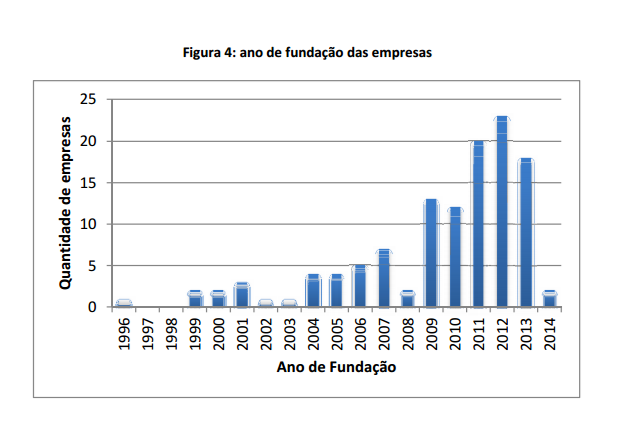
\includegraphics[scale = 0.80]{Imagens/AnoFundacaoEmpresas.png}
    \\ Fonte: Gráfico retirado de \cite{GEDIGames}.
\end{figure}
%
%
%
\par
Com o crescimento da área de desenvolvimento de jogos eletrônicos, surge também a necessidade de encontrar mão-de-obra capacitada, necessidade essa que é uma das maiores reclamações das indústrias de desenvolvimento de \textit{games} do Brasil. Por se tratar de uma área nova, é difícil encontrar profissionais capacitados nela. Uma das soluções mais simples para essa carência de mão-de-obra é incentivar estudantes, sejam eles de nível técnico ou universitário, a aprender sobre as ferramentas e técnicas mais utilizadas no desenvolvimento de um jogo eletrônico. Assim, torna-se de suma importância a implementação de ferramentas que facilitem o primeiro contato do estudante com essa complexa área, motivo esse que motivou a criação da \textit{SAGA Game Library}.
%
%
% ----------------------------------------------------------------
% Objetivos *******************
% ----------------------------------------------------------------
\section{Objetivos}
\label{section:objetivos}
%
A \textit{SAGA Game Library} foi desenvolvida tendo em foco o meio acadêmico. Com o aumento do mercado de desenvolvimento de jogos eletrônicos no país, surge a necessidade de investir na capacitação de profissionais, para atender a essa demanda. Não apenas profissionais do setor precisam estar em constante atualização, mas os agora estudantes e futuros profissionais também precisam de capacitação. É para esse último que é direcionada essa biblioteca. Seu objetivo primário é possibilitar ao usuário, seja ele um estudante ou entusiasta, o primeiro contato com o mundo do desenvolvimento de jogos.
%
\par
%
É certo que já existem muitas \textit{game engines}, inclusive em C++, mas o estudo é o piso de todas as descobertas científicas, o que justifica e motiva o desenvolvimento de uma biblioteca de jogos didática. Esta é a nossa proposta: uma camada de orientação a objetos envolvendo a Allegro de uma forma simples e didática. Simplicidade, eficiência e aprendizado são as palavras-chave da \textit{SAGA Game Library}.
%
%
%